\section{Continuous symmetries}
\label{s:symm}

A dynamical system $\dot{\ssp}=\vel(\ssp)$ is said to be
\emph{equivariant} under the group \Group\ of symmetry transformations if
%                                                \toCB
\beq
	\vel( \ssp )
    =  \matrixRep(\LieEl)^{-1}\vel(\matrixRep(\LieEl)\ssp)
	\,
\ee{equiv}
for every point $\ssp$ in the \statesp\ $\pS$ and every element $\LieEl \in
\Group$, where \LieEl\ is an abstract group element and
$\matrixRep(\LieEl)$ is its $[d\!\times\!d]$ matrix representation.
Infinitesimally, the equivariance condition \refeq{equiv} can be expressed as
a vanishing Lie derivative\rf{DasBuch}
%                                                \toCB
\beq
  \Lg \, \vel(\ssp)  - \Mvar(\ssp) \, \groupTan(\ssp) =0
  \,,
\ee{inftmInv}
where
$\Mvar(\ssp)$ is the $[d\!\times\!d]$ \stabmat\, with elements
$\Mvar_{ij}(\ssp)={\pde \vel_i}/{\pde\ssp_j}|_{\ssp}$, $ \groupTan(\ssp)
= \Lg \ssp $ is the group tangent at $\ssp$, and $\Lg$ is the
$[d\!\times\!d]$ generator of infinitesimal transformations, such that
$\matrixRep(\theta) = \exp(\theta\Lg)$, where the phase $\theta \in [0,2\pi)$
parametrizes the group action. (We shall interchangeably use notations
$\matrixRep(\LieEl)$ and $\matrixRep(\theta)$.) In general, there is a
generator associated with each continuous symmetry. For the simple model 
considered here, which has a single $\SOn{2}$ symmetry, there is only one 
parameter $\theta$, so we only have one generator \Lg.

If the trajectory of a point $\ssp_\stagn$ coincides with its group
orbit, \ie, for every $\zeit$ there is a group transformation such that
\beq
\ssp (\zeit)
    = \ssp_\stagn + \int_0^\zeit \!\!d\zeit' \vel(\ssp (\zeit'))
    = \matrixRep(\theta (\zeit))\,\ssp_\stagn
  \,,
\ee{releq}
$\ssp_\stagn$ is a point on \emph{\reqv} $\stagn$. In our case, this is a 
1-torus in \statesp. Expanding both sides of \refeq{releq} for infinitesimal time
verifies that the group tangent and the velocity vector are parallel, i.e.,
%  need this written out step-by-step in ChaosBook                  \toCB
 $\vel(\ssp_\stagn) = \dot{\theta}(0) \, \groupTan(\ssp_\stagn)$.
By symmetry, this must hold for all $\ssp(\zeit) \in q$, so for \reqva\
the \emph{\phaseVel} is constant, $\dot{\theta}(\zeit) = \velRel$.
Multiplying the equivariance condition \refeq{inftmInv} by $\velRel$, we
find that velocity is a marginal stability eigenvector in the reference frame co-moving 
with the \reqv,
\beq
(\Mvar (\ssp) - \velRel \Lg) \vel (\ssp) = 0
\,,\qquad \ssp \in \pS_\stagn
\,.
\ee{ReqvMargEig}

A \statesp\ point $\ssp_\rpprime$ lies on a \emph{\rpo} of period
$\period{\rpprime}$ if its trajectory first intersects its group orbit after
a finite time $\period{\rpprime}$,
%                                                \toCB
\beq
\ssp(\period{\rpprime})
    = \ssp_\rpprime
     + \int_0^\period{\rpprime} \!\!\!\!d\tau' \vel(\ssp (\tau'))
    = \matrixRep(-\theta_\rpprime) \,  \ssp_\rpprime
  \,,
\ee{relpo}
with a non-zero phase $\theta_{\rpprime}$.\DB{2014-11-16}{Why does the phase have a
minus sign here but a plus sign for relative equilibria above? Is the notational asymmetry
really necessary?}
\BB{2015-01-15}{The negative sign for the \rpo\ is consistent with the
definition of the Jacobian \refeq{e-rpoJacobian} and the Newton method 
in the appendix. I agree that it looks awkward, but once we change this
sign, then we need to change the definition of the Jacobian, and then the 
Newton section, which is very risky. I'll think for a day, and probably 
give up do this tomorrow.}
In systems with \SOn{2}
symmetry, \rpo s are topologically 2-tori, where the trajectory of
$\ssp_\rpprime$ generically traces out the torus ergodically by
repeating the same path shifted by the group action
$\matrixRep(\theta_\rpprime)$ after each prime period
$\period{\rpprime}$. As we will see in \refsect{s:numerics}, these tori
can be very convoluted and difficult to visualize. In special cases where
$\theta_{\rpprime}=0$, the solution is a \po, a 1-dimensional loop in \statesp\ and
the 2-torus is generated by all actions of the symmetry group on this
loop.

The linear stability of \rpo s is captured by their \emph{Floquet
multipliers}  $\ExpaEig_{p,j}$, the eigenvalues of the time-forward map
$\ssp(\zeit)=\flow{\zeit}{\ssp(0)}$ Jacobian
\beq
\jMpsRed_{\rpprime}
= \matrixRep(\theta_\rpprime ) \jMps^\period{\rpprime} (\ssp_\rpprime)
\,, \; \mbox{~where~}\;
\jMps^{\zeit}_{ij} (\ssp(0)) = \frac{\partial\ssp_i(\zeit)}{\partial\ssp_j(0)}\, .
\ee{e-rpoJacobian}
The magnitude of $\ExpaEig_{p,j}$ determines whether a small perturbation
along its corresponding eigendirection (or Floquet vector) will expand or
contract after one period. If the magnitude of $\ExpaEig_{p,j}$ is
greater than $1$, the perturbation expands; if it is less than $1$, the
perturbation contracts. In systems with $N$ continuous symmetries, \rpo s
have $(N+1)$ marginal directions ($\left|\ExpaEig_{p,j}\right| = 1$),
which correspond to the temporal evolution of the flow and the $N$
symmetries. By applying symmetry reduction, the marginal Floquet
multipliers corresponding to the symmetries are replaced by $0$, so that 
periodic orbit theory, which requires that the flow have only one
marginal direction, becomes applicable.

\emph{Symmetry reduction} is a coordinate transformation that maps
all the points on a group orbit $\matrixRep(\theta) \ssp$, which are
equivalent from a dynamical perspective, to a single representative point in a symmetry reduced space.
After symmetry reduction, \reqva\ and \rpo s are converted to \eqva\ and \po s in a
reduced \statesp without loss of dynamical information; the full \statesp\
trajectory can always be retrieved via a reconstruction equation. 

\DBedit{One well-studied technique for symmetry reduction, which works well for low-dimensional
dynamical systems, such as the Lorenz system, is to recast the dynamical equations in terms 
of invariant polynomials\rf{GL-Gil07b}. Establishing such invariant polynomial bases, however, 
quickly becomes impractical for systems with more than a dozen dimensions\rf{gatermannHab}. In contrast,
the \mslices\ \rf{rowley_reconstruction_2000,BeTh04,SiCvi10,FrCv11,atlas12,ACHKW11,BudCvi14},
which we study in detail here, is a symmetry reduction scheme applicable to
high-dimensional flows like the \NS\ equations\rf{WiShCv14}.}\DB{2014-11-16}{This paragraph seems like weird
filler. It might make more sense to move these sentences to the relevant sections below... Thoughts?}

\subsection{\Mslices}
\label{s-slice}

In a system with $N$ continuous symmetries, a \emph{\slice} \pSRed\ is a codimension $N$ submanifold
of \pS\ that cuts every group orbit once and only once. In the \emph{\mslices}, the solution
of a $d$-\dmn\ dynamical system is represented as a symmetry-reduced trajectory $\sspRed (\zeit)$ within the
$(d-N)$-\dmn\ \slice\ and $N$ time dependent group parameters $\theta(\zeit)$, which
map $\sspRed (\zeit)$ to the full \statesp\ by the group action $\matrixRep(\theta(\zeit))$.

While this idea goes back to Cartan\rf{CartanMF},
it was first used to study spatially-extended nonlinear flows by Rowley and Marsden\rf{rowley_reconstruction_2000}. 
They used it to study the dynamics of
the $1D$ \KS\ equation in the neighborhood of
a \reqv by using the \reqv\ itself as the \slice\ `\template'.
Independently, Beyn and Th\"{u}mmler\rf{BeTh04} applied
the \mslices\ to `freeze' spiral waves in reaction-diffusion systems.

The definition of a \slice\ given above puts no restriction on its shape
and offers no guidance on how to construct it. In practice, a
local approximation of the slice called a \emph{\slicePlane} can be constructed
in the neighborhood of a point $\slicep$ by using $\slicep$ as
\emph{\template}. The \slicePlane\ is then defined as the hyperplane that
contains $\slicep$ and is perpendicular to its group tangent $\sliceTan{}
= \Lg \slicep$. The relationship between a \template, its \slicePlane, and symmetry-reduced trajectories
is illustrated in \reffig{f-ReducTraj1}.

%% ReducTraj*.* - read dasbuch/book/FigSrc/inkscape/00ReadMe.txt
\begin{figure}
\begin{center}
 \setlength{\unitlength}{0.40\textwidth}
 %% \unitlength = units used in the Picture Environment
 \begin{picture}(1,0.8361641)%
   \put(0,0){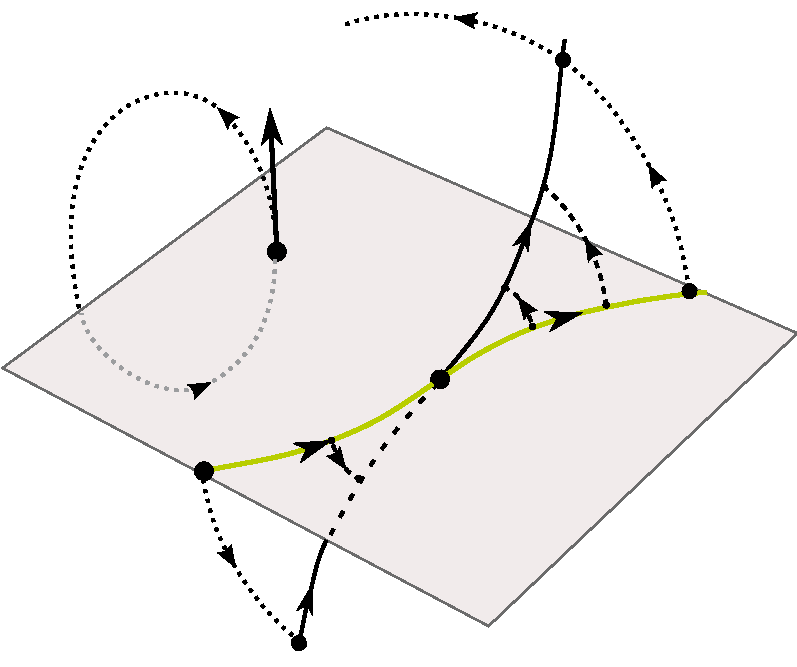
\includegraphics[width=\unitlength]{ReducTraj5.pdf}}%
   \put(0.55,0.07){\color[rgb]{0,0,0}\rotatebox{-30.34758661}{\makebox(0,0)[lb]{\smash{$\pSRed$}}}}%
   \put(0.57768586,0.29773425){\color[rgb]{0,0,0}\rotatebox{0.0313674}{\makebox(0,0)[lb]{\smash{$\sspRed(0)$}}}}%
   \put(0.59310014,0.69932675){\color[rgb]{0,0,0}\rotatebox{0.03136739}{\makebox(0,0)[lb]{\smash{$\ssp(\zeit)$}}}}%
   \put(0.8268425,0.39772328){\color[rgb]{0,0,0}\rotatebox{0.03136739}{\makebox(0,0)[lb]{\smash{$\sspRed(\zeit)$}}}}%
   \put(0.81220962,0.66529577){\color[rgb]{0,0,0}\rotatebox{0.03136739}{\makebox(0,0)[lb]{\smash{$\matrixRep(\theta(\zeit))\sspRed(\zeit)$}}}}%
   %\put(0.21150193,0.63610779){\color[rgb]{0,0,0}\rotatebox{0.0313674}{\makebox(0,0)[lb]{\smash{$\matrixRep(\theta)\,\slicep$}}}}%
   \put(0.37740434,0.49597258){\color[rgb]{0,0,0}\rotatebox{0.0313674}{\makebox(0,0)[lb]{\smash{$\slicep$}}}}%
   \put(0.3627714,0.69665188){\color[rgb]{0,0,0}\rotatebox{0.0313674}{\makebox(0,0)[lb]{\smash{$\sliceTan{}$}}}}%
 \end{picture}%
\end{center}
\caption{\label{f-ReducTraj1}
(Color online) The \slicePlane\ \pSRed\ is a hyperplane that contains 
the {\template} point $\slicep$ is and normal to its group
tangent $\sliceTan{}$. It intersects all group orbits (dotted lines) in
an open neighborhood of $\slicep$. The full \statesp\ trajectory
$\ssp(\tau)$ (solid black line) and the \reducedsp\ trajectory
$\sspRed(\zeit)$ (dashed green line) belong to the same group orbit
$\pS_{\ssp(\zeit)}$ and are equivalent up to a group rotation
$\matrixRep(\theta(\zeit))$.
}%
\end{figure}

Reduced trajectories $\sspRed (t)$ can be obtained in two ways: by
post-processing data or by reformulating the dynamics and integrating
directly in the \slicePlane. The post-processing method (also called the
\emph{method of moving frames}\rf{FelsOlver98,OlverInv}) can be applied
to both numerical and experimental data, one takes the data in the full
\statesp\ and looks for the time dependent group parameter that brings
the trajectory $\ssp(\zeit)$ onto the \slice. That is, one finds $\theta
(\zeit)$ such that $\sspRed(\zeit)=\matrixRep(-\theta (\zeit)) \ssp
(\zeit)$ satisfies the \slice\ condition:
\beq
\braket{\sspRed(\zeit) - \slicep}{\sliceTan{}} = 0
\,.
\ee{SliceCond}

In the second implementation, one reformulates the dynamics (for Abelian
groups) as
\begin{subequations}\label{eq:so2reduced}
  \beq\label{eq:intSlice}
	\velRed(\sspRed) = \vel(\sspRed)
	-\dot{\theta}(\sspRed) \, \groupTan(\sspRed)
  \eeq
  \beq\label{eq:reconstruction}
	\dot{\theta}(\sspRed) = {\braket{\vel(\sspRed)}{\sliceTan{}}}/
				{\braket{\groupTan(\sspRed)}{\sliceTan{}}}
  \, ,
  \eeq
\end{subequations}
which can then be directly integrated to get the symmetry-reduced trajectory $\sspRed (\zeit)$ and the reconstruction angle $\theta (\zeit)$.
In \refeq{eq:so2reduced}, $\velRed$ is the projection of the full \statesp\ velocity \vel(\ssp) onto the \slicePlane.
For a derivation of \refeq{eq:so2reduced}, see \refref{DasBuch}.

While early studies\rf{rowley_reconstruction_2000, rowley_reduction_2003,
BeTh04} applied the \mslices\ to a single solution at a time, studying
the nonlinear dynamics of extended systems requires symmetry reduction of
global objects, such as strange attractors or invariant manifolds. In
this spirit, Siminos and Cvitanovi\'{c}\rf{SiCvi10} used the \mslices\ to
quotient the \SOn{2} symmetry from the chaotic dynamics of \cLf. They
showed that the singularity of the reconstruction
equation that occurs when the denominator in \refeq{eq:reconstruction}
vanishes (e.g., when the group tangents of the trajectory and the
template are orthogonal) causes the reduced flow to make discontinuous
jumps. The set of points $\sspRed^*$ where this occurs satisfy
\beq
\braket{\groupTan(\sspRed^*)}{\sliceTan{}} = 0
\ee{ChartBordCond}
and make up the \emph{\sliceBord}, which was studied in detail by Froehlich and Cvitanovi\'{c}\rf{FrCv11}.

Two strategies have been proposed in order to handle this problem: The first attempts to
try to identify a template such that slice singularities are not visited
by the dynamics\rf{SiCvi10}. The second uses multiple `charts' of connected
\slicePlane s\rf{rowley_reconstruction_2000,FrCv11}, switching between charts when the
dynamics approach the border of a particular chart. The latter approach was applied to \cLf\ by Cvitanovi\'{c} \etal~\rf{atlas12} and
to pipe flow by Willis, Cvitanovi\'{c}, and Avila\rf{ACHKW11}.
However, neither approach is straightforward to apply, particularly to
high-dimensional systems.

\subsection{\FFslice}
\label{sect:fFslice}

A third strategy has recently been proposed by Budanur
\etal\rf{BudCvi14}, who considered Fourier space discretizations of
partial differential equations (PDEs) with \SOn{2} symmetry. They showed
that in these cases a simple choice of \slice\ template, associated with
the first Fourier mode, results in a \slice\ in which it is highly
unlikely that generic dynamics visit the neighborhood of the singularity.
If the dynamics do occasionally come near the singularity, these close
passages can be regularized by means of a time rescaling.

Here, we shall illustrate this approach, which we call the `\fFslice',
and apply it to a model system with two modes that will be described in \refsect{s:twoMode}.
This model is arguably one of the simplest systems with \SOn{2} equivariant dynamics that can
exhibit chaos.

In the discussion so far, we have not specified any constraints on the symmetry group
to be quotiented beyond the requirement that it be Abelian as required for \refeq{eq:so2reduced}
to be valid.\ES{2015-05-20}{Maybe you should discuss why
you imposed the restriction on Abelian groups.} Since we are interested in spatially extended systems with
translational symmetry, and in order to keep the notation compact,
we restrict our discussion to one dimensional PDEs describing
the evolution of a field $u(x,t)$ in a periodic domain.
By expressing the solutions in terms of a Fourier series
\beq
	u(x,\zeit) = \sum\limits_{k=- \infty}^\infty u_k\left(\zeit\right) e^{i k x}, \,\,\,u_k = x_k + i y_k,
\ee{FourierSeries}
the translationally invariant PDE can be replaced by a system of coupled nonlinear
ODEs for the Fourier coefficients equivariant under the 1-parameter compact group of \SOn{2} rotations.

Truncating the expansion to $m$ modes, we write the real and imaginary
parts of the Fourier coefficients with $k \geq 1$ as the state vector
$\ssp=\cartpt{x_1, y_1, x_2, y_2,..., x_m, y_m}$. The action of the
$\SOn{2}$ group on this vector can then be expressed as a block diagonal
matrix:
\beq
	\matrixRep(\theta) = \begin{pmatrix}
						R(\theta) & 0 			  & \cdots & 0 \\
						0		   & R(2 \theta) & \cdots & 0 \\
						\vdots	   & \vdots 	  & \ddots & \vdots \\
						0		   & 0	          & \cdots & R (m \theta)
					   \end{pmatrix}
\,,
\ee{mmodeLieEl}
where
\beq
	R(n \theta) =	\begin{pmatrix}
					\cos n \theta & - \sin n \theta \\
					\sin n \theta & ~\cos n \theta
					\end{pmatrix}
\ee{rotationmatrix}
is the rotation matrix for $n$th Fourier mode.
The Lie algebra generator for $\matrixRep(\theta)$ is given by
\beq
	 \Lg =  \begin{pmatrix}
			 0 & -1 & 0 & 0 & \cdots & 0 & 0 \\
			 1 & 0 & 0 & 0 & \cdots & 0 & 0 \\
			 0 & 0 & 0 & -2 & \cdots & 0 & 0 \\
			 0 & 0 & 2 & 0 & \cdots & 0 & 0 \\
			 \vdots & \vdots & \vdots & \vdots & \ddots & \vdots & \vdots \\
			 0 & 0 & 0 & 0 & \cdots & 0 & -m \\
			 0 & 0 & 0 & 0 & \cdots & m & 0
			 \end{pmatrix} .
\ee{mmodeLg}

In order to construct a \slicePlane\ for such a system, we choose the
following \slice\ \template:
\beq
	\slicep = (1, 0, ..., 0) .
\ee{firstmodetemp}
The \slice\ condition \refeq{SliceCond} then constrains points on the
reduced trajectory to the hyperplane given by
\beq
	\sspRed = (\hat{x}_1, 0, \hat{x}_2, \hat{y}_2, ..., \hat{x}_m, \hat{y}_m) .
\ee{slicetemp}
As discussed earlier, group orbits should cross the \slice\ once and only
once, which we achieve by restricting the \slicePlane\ to the half-space
where $\hat{x}_1 > 0$. In general, a \slicePlane\ can be constructed by
following a similar procedure for any choice of \template. However, the power of
choosing template \refeq{firstmodetemp} becomes apparent by computing the
border \refeq{ChartBordCond} of its \slicePlane. The points on \refeq{slicetemp} lie on the
\sliceBord\ only if $\hat{x}_1 = 0$. This means that as long the dynamics
are such that the magnitude of the first mode never vanishes,
\emph{every} group orbit is guaranteed to have a unique representative
point on the \slicePlane. By symmetry, any template of the form $\slicep
=\cartpt{\hat{x}'_1, \hat{y}'_1, 0,...,0}$  would work just as well. The
\slice\ \template\ \refeq{firstmodetemp} was chosen for notational and
computational convenience.

More insight can be
gained by writing the symmetry-reduced evolution equations \refeq{eq:so2reduced}
explicitly for the template \refeq{firstmodetemp}:
\begin{subequations}
\beq
\velRed ( \sspRed )  = \vel(\sspRed)
   - \frac{\dot{y}_1\left(\sspRed\right)}{\hat{x}_1} \, \groupTan(\sspRed) \, ,
\label{e-so2red1stmode}
\eeq
\ESedit{
  \beq\label{eq:reconstruction1stmode}
	\dot{\theta}(\sspRed) = \frac{\dot{y}_1(\sspRed)}{\hat{x}_1}
  \, .
  \eeq
}
\end{subequations}
Since the argument $\phi_1$ of a point $(x_1,y_1)$ in the first Fourier mode plane is given by $\phi_1=\tan^{-1}\frac{y_1}{x_1}$,
its velocity is
\beq
  \dot{\phi}_1 = \frac{x_1}{r_1^2}\dot{y}_1-\frac{y_1}{r_1^2}\,\dot{x}_1\,,
\eeq
where $r_1^2=x_1^2+y_1^2$. Therefore, on the \slicePlane\ \refeq{slicetemp}, where $\hat{y}_1=0$,
\beq\label{eq:phi1}
  \dot{\theta}(\sspRed) = \dot{\phi}_1(\sspRed)\,.
\eeq
That is, for our choice of \template\ \refeq{firstmodetemp}, the
reconstruction phase coincides with the phase of the first Fourier mode. This makes this choice of template 
more natural from a group-theoretic point of view than the physically motivated templates used in
\refrefs{rowley_reconstruction_2000,BeTh04,SiCvi10,FrCv11,atlas12,ACHKW11}.

\ES{2014-05-20}{What would you think about introducing a functional
notation for $y_1$ as in \refeq{eq:reconstruction1stmode}?}
\PC{2014-05-25: We should copy and paste from \refref{BudCvi14} all stuff
about the in-slice time here? }
\ES{2014-05-25}{I agree with that suggestion, since rescaled time makes the
method work for more general flows than 2-modes,
and it should be explained here. However, we do not provide an example for it's
usefulness here. How about fishing for a second set of parameters where
trajectories come consistently close to $(0,0,\ldots)$, and using rescaled
time there? Even though $(0,0,\ldots)$ would not be visited, there should still
be apparent jumps that would go away by time-rescaling.}
In general, additional care must be taken when the dynamics approach the \slice\ border $\hat{x}_1 = 0$.
Whenever this happens, the near-divergence of $\velRed$ can be regularized by introducing a rescaled time coordinate such that
$d\hat{\zeit} = d\zeit / \hat{x}_1$\rf{BudCvi14}. However, in our analysis of the \twomode\ system that we introduce below,
we omit this step since points with a vanishing first mode are in an invariant subspace of the flow and, hence, are never
visited by the dynamics.

\subsection{Geometric interpretation of the first Fourier mode \slice}
\label{s-mframes}

\begin{figure}%[H]
\centering
 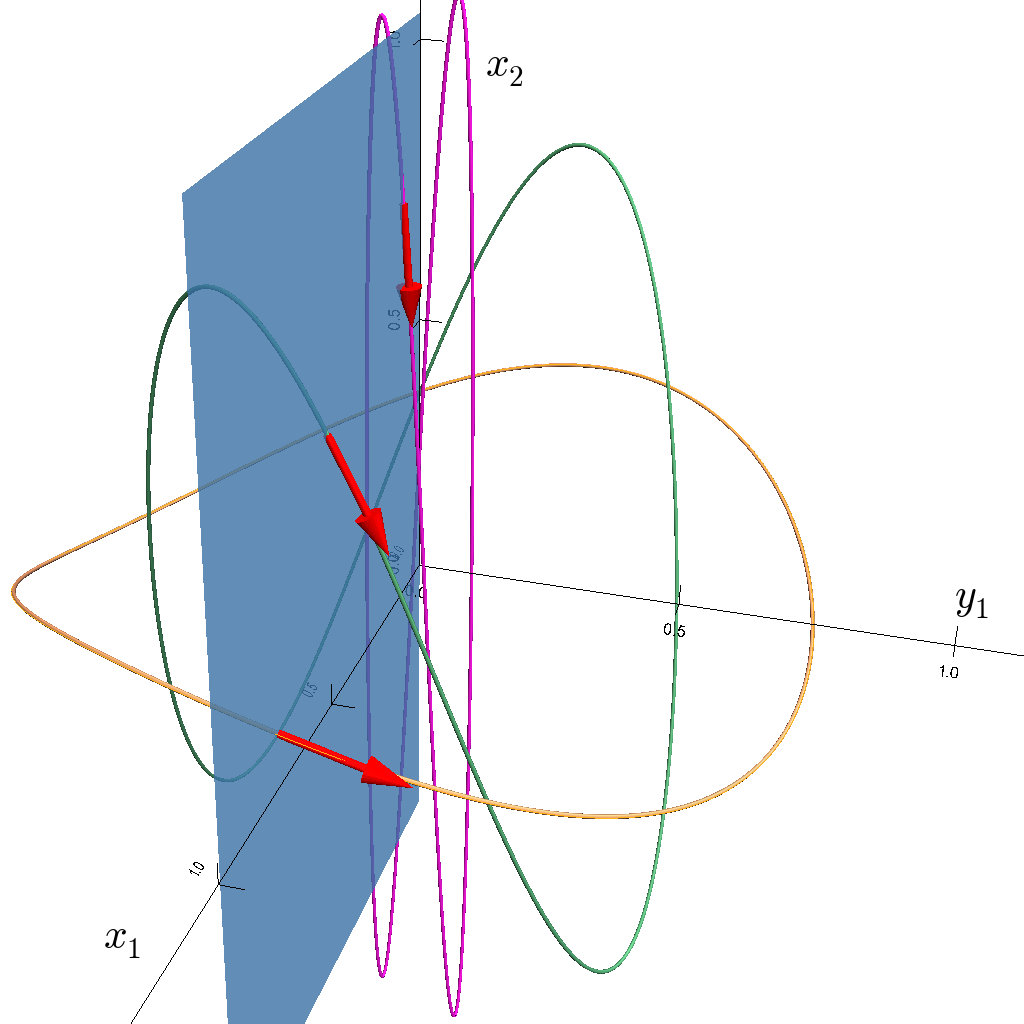
\includegraphics[width=0.45\textwidth]{BBgorbitsandslice}
\caption{(Color online)
$\SOn{2}$ group orbits of \statesp\ points $\cartpt{0.75, 0, 0.1, 0.1}$
(orange), $\cartpt{0.5, 0, 0.5, 0.5}$ (green)
$\cartpt{0.1, 0, 0.75, 0.75}$ (pink) and the first mode \refeq{slicetemp} \slicePlane\
(blue). The group tangents at the intersections with the
\slicePlane\ are shown as red arrows.
As the magnitude of the first Fourier mode decreases relative to the
magnitude of the second one, so does the group tangent angle to the
\slicePlane.}
\label{fig:BBgorbitsandslice}
\end{figure}

Before moving on to our analysis of the \twomode\ model, we first discuss the geometrical
interpretation of the first Fourier mode \slice. The \slice\ defined by \refeq{firstmodetemp}, along with the directional constraint
$\hat{x}_1 > 0$,
%
\DB{2014-05-15}{Think this should be $\hat{x}_1$. Revert to $x_1$ if I'm wrong.}
%
fixes the phase of the first complex Fourier mode to $0$. This can also be seen
from \refeq{eq:phi1}, which shows that if the first Fourier mode \slice\ \refeq{firstmodetemp} is used as 
a \template, the reconstruction phase \refeq{} is the same as the phase of the first 
Fourier mode \refeq{eq:phi1}. 

In complex representation, we can express the relationship
between Fourier modes ($\sspC_n = x_n + \ii y_n$) and their
representative points ($\sspRedC = \hat{x}_n +  \ii \hat{y}_n$) on the
\slicePlane\ by the $\Un{1}$ action:
\beq
	\sspRedC_n = e^{-\ii n \phi_1} \sspC_n \, . \ee{e-1stmodeTransform}
This relation provides another interpretation for the \sliceBord:  For
template \refeq{firstmodetemp}, the \sliceBord\ condition
\refeq{ChartBordCond} defines the \sliceBord\ as those points where $|\sspRedC_1| = |\sspC_1| = 0$.
At these points the phase of the first Fourier mode is not well-defined and hence 
neither is the transformation \refeq{e-1stmodeTransform}.

This is illustrated in \reffig{fig:BBgorbitsandslice}, where the
first Fourier mode \slicePlane\ is shown along with the group orbits of points 
with decreasing $|\sspC_1|$. When the magnitude of the first mode is small 
relative to that of the second (pink curve in
\reffig{fig:BBgorbitsandslice}), the group tangent at the representative point for 
the group orbit (i.e., where the group orbit and the \slicePlane\ intersect) has a larger component
parallel to the \slicePlane. If the magnitude of the first mode was exactly
$0$, the group tangent would lie entirely on the \slicePlane , satisfying
the \sliceBord\ condition.

In \refref{PoKno05}, a polar coordinate representation of two Fourier mode
truncation is obtained by defining the $\Group$-invariant phase: $\Phi = \phi_2 - 2 \phi_1$
and three symmetry invariant coordinates \polpt{r_1, r_2 \cos \Phi, r_2 \sin \Phi}.
One can see by direct comparison with \refeq{e-1stmodeTransform}, which
yields $\sspRedC_1 = r_1$ and $\sspRedC_2 = r_2 e^{\ii \Phi}$, that this
representation is a special case $(m=2)$, of the \slice\ defined by
\refeq{firstmodetemp}. Corresponding ODEs for the polar representation
were obtained in \refref{PoKno05} by  chain rule and substitution. Note
that \mslices\ provides a general form \refeq{e-so2red1stmode} for symmetry
reduced time evolution.\DB{2014-10-28}{This section is kind of weird... doesn't seem to flow and we don't really use this stuff anywhere. Maybe consider deleting.}
\BB{2014-10-30}{In \refref{PoKno05} they use this representation and their plots
of chaotic dynamics (yes, they have parameters for which the \twomode\ system exhibits
chaos) look very similar to ours. We have to state somewhere that this similarity
is not an accident. I agree that it looks awkward as an individual subsection,
I removed the subsection title for now, we may move it to the `flow' section.} \DB{2015-1-9}{Yeah... this definitely needs to go somewhere else... 
maybe where we discuss invariant polynomials since this is a coordinate transform that works because this system is easy but would never work
for Navier-Stokes.}
